\documentclass[11pt, oneside]{article}   	% use "amsart" instead of "article" for AMSLaTeX format
\usepackage{geometry}                		% See geometry.pdf to learn the layout options. There are lots.
\geometry{letterpaper}                   		% ... or a4paper or a5paper or ... 
%\geometry{landscape}                		% Activate for rotated page geometry
%\usepackage[parfill]{parskip}    		% Activate to begin paragraphs with an empty line rather than an indent
\usepackage{graphicx}				% Use pdf, png, jpg, or eps§ with pdflatex; use eps in DVI mode
								% TeX will automatically convert eps --> pdf in pdflatex		
\usepackage{amssymb}

\usepackage{fancyhdr}
\fancyhead[L]{DATE}
\fancyhead[C]{SE 3XA3 Test Plan}
\fancyhead[R]{Genzter}
\pagestyle{fancy}

\usepackage{float}

\usepackage{hyperref}

%SetFonts

%SetFonts


\title{Test Plan: Revision 0}
\author{Group 2 - Genzter \\
		\\ Binu, Amit - binua - 400023175
		\\ Bengezi, Mohamed - bengezim - 400021279
		\\ Samarasinghe, Sachin - samarya - 001430998
		\\ October 27, 2017
		\\Professor: Dr. Bokhari
		\\ Lab: L01}

\begin{document}
\maketitle

\newpage
\section{Revision History}

\begin{table}[h]
\begin{center}
\begin{tabular}{ | c | c | c | c | }
\hline
 Date & Version & Description & Author \\ 
\hline
 05/OCT/17 & 0.0 & Created Test Plan & Mohamed Bengezi, Amit Binu, Sachin Samarasinghe \\  
\hline
  & & & \\
\hline
 & & & \\
\hline 
 & & & \\ 
\hline 
\end{tabular}
\end{center}
\caption{Revision History}
\end{table}

\newpage
\tableofcontents
\listoffigures
\listoftables

\newpage
% INTRODUCTION
\section{Introduction}
\subsection{Purpose}
The goal of this project is to create a viable set of schedules for the user based on the inputted courses. All correcponding core's, labs, and tutorials must be included in each timetable. The automated testing shall include unit testing performed by the Mocha framework for javascript. Functional testing shall consist of input testing, along with conflict tests, and perfect input tests. Structural testing shall inlcude performance tests, such as a large number of courses as input, as well as dataset traversal tests. Fault and Mutation testing will occur throughout development. Manual testing, such as static testing, shall be done primarily by group code walkthrough's \& inspections, in order to check syntax and logic, and gain a better understanding of the program code as a whole. Dynamic testing shall include using a number of predetermined schedules from various programs, and using the courses on each schedule as input, and determining that each necessary core, lab, and tutorial are listed in the generated timetable. 

\subsection{Objectives}
This test plan will allow the team to head into the testing phase in an organized and informed manner, and with a clear goal in mind. These tests ensure that the product will be working as it should be when released for users. The plan will also ensure that testing is conducted properly, and any interested parties can learn about the testing of the product.\

\subsection{References}
Project inspiration: \url{http://timetablegenerator.io} \\
Open sourced similar project: \url{https://github.com/ash47/TimetableGenerator}

\newpage



% PLAN
\section{Plan}
\subsection{Software Description}
The program uses Node js for the backend, and HTML/CSS for the front end. The main modules in the program are the index.js module, which contains the code for the main page, the checkCourse.js module, which checks and  ensures all user inputs are valid and viable, the scheduler.js module, which is the main algorithm for creating the timetables, the Course.js module, which defines the course objects used throughout the program, and all the corresponding ejs files, which contain the HTML code for the front end of each page. 
%%%%%%%%%%%%%%%%%%%%%%%%%%%%%%

\begin{figure}[H] %  figure placement: here, top, bottom, or page
   \centering
   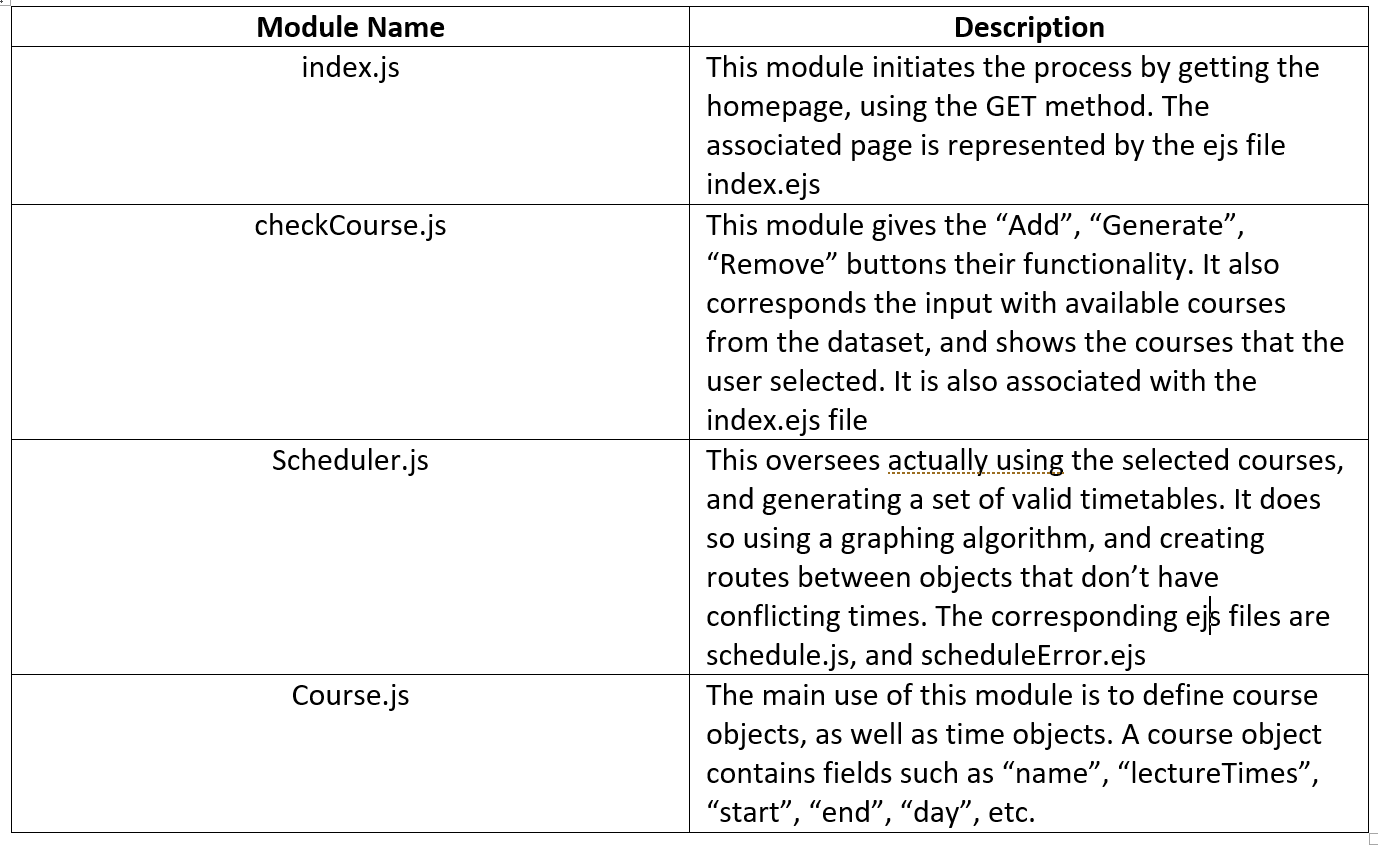
\includegraphics[width=5in]{Software_Description.png} 
   \caption{Software Description}
   \label{}
\end{figure}


\subsection{Test Team}
The entire Genzter team will be in tasked with testing. Testing shall be evenly divided between members.

\subsection{Automated Testing Approach}
As stated above, automated testing will be done using the javascript testing framework called \href{http://mochajs.org}{Mocha}. Accompanying Mocha will be an assertion library called \href{http://chaijs.com/}{Chai}. Unit tests will be set up, and the framework will be used to automatically run through all the unit tests, and reveal any faults that may reside in the program. The unit tests will include normal input, boundary cases, as well as extreme cases and conflicting cases. This will ensure that the program functions expectedly, and that no special cases were missed. In other words, this automated testing approach will make sure that in any case, the program will have a path to follow, and its behaviour can be predicted.

\subsection{Testing Tools}
For unit testing we will be using the testing framework \href{http://jasmine.github.io/}{Jasmine}. For system testing we will be running the game by executing it on a browser and observing the functionalities. For code analysis we will use humans with coding experience to analyze the code.

\subsection{Testing Schedule}
The testing schedule is included in the
 
\subsection{Testing: Primary}
The software that will be required is a JavaScript automated testing framework, a server that can host our website when we're testing on different devices and browsers, a text editor that can make changes to specific pieces of code that will require changing, and a media editor that will be able to modify images and change signs. 
The required personnel to set-up automated testing will be required to have sufficient knowledge in JavaScript and HTML to setup multiple test cases. However, users and development groups that will be doing manual testing do not not have specific requirements needed for testing. 
The automated testing will be done through Jasmine Framework that provides its own documentation. It creates cases that require inputs and expected outputs and will allow the tester to find faults if any. It will create webpages with documentation that show whether a test case has passed or failed and why. 
The proof of concept will indicate correct sound output and frame resizing. It will display a simple test run through the Jasmine Framework showing that both functions are ideal in their outputs. This testing will then be shown and used as a guideline to other tests. 
\\
\\
\\

\subsection{Testing: Secondary}
Secondary testing will be done by users in our open beta testing. We will allow users to access our game at an early development stage after preliminary tests by developers. They will be able to manually perform functional testing by checking for bugs and running through the game through our website. 

\newpage
% SPECIFICATIONS AND EVALUATION
\section{Specifications and Evaluation}
\subsection{Specifications}
\subsubsection*{Business Functions}
\begin{itemize}
\item The executable HTML file will create a new browser window.

\item The HTML will be executed by a browser with JavaScript functionality.

\item The game will have a standby state in which it waits for user input.

\item Upon the reception of user input from the standby state the game will begin.

\item At the beginning of the game the user will perceive all stats reset to their default state.

\item At the beginning of the game the user character will maintain its state until user input is received.

\item If there is a collision with the user character and an obstacle object the game will terminate and all stats will be recorded.

\item Upon termination of the game state all stats will be reset to their default state and the standby state will be reinitiated.

\item If there is a collision with the user character and an objective object the user's score will increment and the objective object's instance will terminate.

\item During the game state reception of user input will cause the user character to respond in a constant and uniform manner relative to the user character's instance.
\end{itemize}

\subsubsection*{Structural Functions}
\begin{itemize}
\item Cookie
\subitem Test how cookies are created and used by the program through static and dynamic testing. This includes code analysis, unit testing, and system testing.

\item Rendering
\subitem Test the use of graphic files compared to drawing objects for the game rendering. This includes manual system testing for aesthetic purposes. 
\end{itemize}

\subsubsection*{Test/Function Relationships}
Much of the testing done for the structural functions will be changed depending on how we (the developers) choose to optimize or design the appearance of the product.\\
\\
For the structural testing of the cookies, it must be decided on which data to store for each cookies instance and how that data will affect the game. This can be done initially through manual code analysis then verified with unit testing, and a manual system test where the value of the cookie can be checked by access through the game and of where the cookies are stored.\\
\\
The structural rendering tests will be used to decide through the aesthetic decisions of the designers and developers the presentation of core functional and ornamental objects in the game. As such the tests conducted will mostly be done through manual system tests although additional unit tests can be performed to validate the functionality of either drawing or using images to render objects.

\subsubsection*{Test Progression}
The tests will proceed by verifying the business functions and all critical components of the project software. With the basis of the project verified structural testing can proceed to optimize the performance of the product and the end users' experience with the product.

\subsection{Methods and Constraints}
\subsubsection*{Methodology}
The A Team's (the developers) approach to testing is to validate the core functionality of the product being developed before testing non-critical components of the product.

\subsubsection*{Test Tools}
For unit testing we will be using the testing framework \href{http://jasmine.github.io/}{Jasmine}. For system testing we will be running the game by executing it on a browser and observing the functionalities. For code analysis we will use humans with coding experience to analyze the code.

\subsubsection*{Extent}
The entirety of the product will be tested.

\subsubsection*{Data Recording}
The results of the unit testing will be written to a test results log. System testing will be added to a separate test log specifcaly for system testing, as will code analysis.\\
\\
All test will contain information on the aspect being tested, the date of the test, the person running the test, the results of the test, a description of the test purpose, a description of the test results, and next steps from the test.

\subsubsection*{Constraints}
Due to the game's simple mechanics, there are few constraints on the testing.

\subsection{Evaluation}
\subsubsection*{Criteria}
Our tests will cover primarily the boundaries of the game mechanics and some testing inside the boundaries as an example test of normal behaviour.

\subsubsection*{Data Reduction}
All test logs will indicate a pass or a need fro review which allow us to focus on reimplementing and testing components which do not pass the tests.

\newpage
% TEST DESCRIPTION
\section{Test Descriptions}
\subsection{Test Identification}
Control: The team are going to be using automatic insertions, in the form of a unit tester named Jasmine. Our team will also manually create non automated inputs in the form of playing the game.\\
\\
The inputs created from Jasmine will be in the three different forms. First will we have Jasmine change the location of our fish player to random locations, and by knowing what spaces are occupied by pipes, the Jasmine Framework can determine when the collision function should return true. Next our inputs will be in the form of Jasmine checking for stored cookies. As a result of some browsers not allowing cookies, this isn't a full proof test and some manual testing will be needed. Lastly, the input going into the input recognition function will be a replica of random inputs a user may put if they were actually playing. If the program registers the input as intended, the program will pass. For the manual testing, our inputs will be the team actually running the game and giving usual and unusual user inputs and seeing how the program reacts.\\
 \\
Manual testing will occur on different browsers such as Chrome, Explorer, Firefox, etc. This will allow diversity within our tests. Automated testing (through Jasmine) will consist of many different sets of inputs. Jasmine will be given a set of expected outputs and will allow a test to pass if these outputs are met given many different inputs. Some tests will attempt to generate exceptions by accessing inputs outside of the alphabet of possible inputs such as accessing cookies that do not exist, etc.\\
\\
The outputs will be pretty straight forward to tell for the Jasmine Framework. If the fish is on the same location that is occupied by a pipe the collision function should return true. The output for the cookie testing will be slightly different, as it will just be a check to see if the cookies were stored. The output for our manual testing will be comprised of images showing the expected results. 

\subsection{Additional Test Identification}
The last of our testing will be semantics and syntax testing. We need for this program to render neatly and look clean. This will be done by trying different frame sizes, different animations and changing the images in our sprite library. Checking this fairly regularly is a smart idea to find the most ascetically pleasing set of sprites and the nicest size to fit our game onto (a preferred size). Variable naming and implementation layouts will be tested to make sure our code is understandable to all members and that the code makes sense to someone trying to maintain it. Syntax will be tested regularly by running the program and having other members look over new additions. This will make sure that we avoid a syntax mistake that could cause problems later down the road for our project and have the team unsure about its location. System tests will be conducted to cross check against the prototype to ensure proper functionality.\\
\\
In addition structural testing will include performance, difficulty, accessibility, and meeting aesthetic requirements. Performance related testing will determine frame rate speeds on differing browsers; server lag and the machine's processing power will be taken into consideration. Difficulty will be adjusted for a subjectively optimal user experience by mutation testing the rendered obstacle functions. The accessibility will be tested by running system tests on different machine types running varying browsers and operating systems per test. Aesthetic requirements will be met through manual system testing by using different sprite designs and will be decided at the discretion of the developers.

\end{document}
